%%%%%%%%%%%%%%%%%%%%%%%%%%%%%%%%%%%%%%%%%%%%%%%%%%%%%%%%%%%%%%%%%
%Tipo de Documento
\documentclass[12pt]{report}

%Paquetes utilizados
\usepackage[letterpaper]{geometry}
\usepackage[myheadings]{fullpage}
\usepackage{fancyhdr}
\usepackage{enumitem}
\usepackage{lastpage}
\usepackage{graphicx, wrapfig, subcaption, setspace, booktabs}
\usepackage[T1]{fontenc}
\usepackage[utf8]{inputenc}
\usepackage[spanish]{babel}
\usepackage[font=small, labelfont=bf]{caption}
\usepackage{fourier}
\usepackage[protrusion=true, expansion=true]{microtype}
\usepackage{sectsty}
\usepackage{url, lipsum}
\usepackage{apacite}
\usepackage{multirow}
\usepackage{caption}
\usepackage{float}
\usepackage{arydshln}
\usepackage{amsmath}
\usepackage{adjustbox}
\usepackage{rotating}
\usepackage{array,tabularx}
\usepackage{longtable}
\usepackage[flushleft]{threeparttable}
\usepackage{pbox}
\usepackage[hidelinks]{hyperref}
\usepackage{pdflscape}


%Comandos especiales
\newcolumntype{C}[1]{>{\raggedright\let\newline\\\arraybackslash\hspace{0pt}}m{#1}}

\makeatletter
\def\adl@drawiv#1#2#3{%
	\hskip.5\tabcolsep
	\xleaders#3{#2.5\@tempdimb #1{1}#2.5\@tempdimb}%
	#2\z@ plus1fil minus1fil\relax
	\hskip.5\tabcolsep}
\newcommand{\cdashlinelr}[1]{%
	\noalign{\vskip\aboverulesep
		\global\let\@dashdrawstore\adl@draw
		\global\let\adl@draw\adl@drawiv}
	\cdashline{#1}
	\noalign{\global\let\adl@draw\@dashdrawstore
		\vskip\belowrulesep}}
\makeatother

\newcommand{\HRule}[1]{\rule{\linewidth}{#1}}
\onehalfspacing
\setcounter{tocdepth}{5}
\setcounter{secnumdepth}{5}


%%%%%PARA ENCABEZADOS Y PIES DEL TEXTO
\pagestyle{fancy}
\fancyhf{}
\setlength\headheight{15pt}
\fancyhead[R]{Centro de Estudios de Conflicto y Cohesión Social}
\fancyfoot[R]{Página \thepage\ de \pageref{LastPage}}



\begin{document}

%%%%TITULO DEL DOCUMENTO

\begin{titlepage}
	\centering
	
\includegraphics[width=16cm]{coes_blanco_esp}

\HRule{1.4pt} \\
\LARGE \textbf{\uppercase{Estudio Longitudinal Social de Chile}}\\
\LARGE \textbf{\uppercase{(ELSOC 2017)}}\\

\HRule{1.4pt} \\ [0.2cm]

\normalsize  \vspace*{0.2\baselineskip}
 \large \textsc{MANUAL DE USUARIO DE BASE DE DATOS\\ 	CORTE TRANSVERSAL}
\\ [0.2cm]
\vspace*{0.9cm}
Editado por:\\
\begin{center}
Roberto González\hspace*{1.25cm}Matías Bargsted\hspace*{1.25cm}Daniel Miranda\\
Benjamín Muñoz\hspace*{1.5cm}Alejandro Plaza\\
\end{center}
\vspace*{1.3cm}
\textbf{Versión 2.0}\\
08 de Enero de  2019\\
\end{titlepage}


%%TABLA DE CONTENIDOS
\tableofcontents
\newpage

%%LISTADO DE FIGURA Y TABLAS
\listoffigures
\listoftables
\newpage

%%%%%FORMATEO DE SECCIONES
	\sectionfont{\scshape}

%%%%%DOCUMENTOS EN SÍ (SECCIONES)

\section*{Presentación}
\addcontentsline{toc}{section}{Presentación}

El Estudio Longitudinal  Social de Chile (ELSOC) es una encuesta desarrollada para analizar intertemporalmente la evolución del conflicto y cohesión en la sociedad chilena, basándose en modelos conceptuales descritos en la literatura nacional e internacional que abordan dichas materias. De este modo, se orienta a examinar los principales antecedentes, factores moderadores y mediadores, así como las principales consecuencias asociadas al desarrollo de distintas formas de conflicto y cohesión social en Chile. Por lo tanto, su objetivo fundamental es constituirse en un insumo empírico para la comprensión de las creencias, actitudes y percepciones de los chilenos hacia las distintas dimensiones de la convivencia y el conflicto, y como éstas cambian a lo largo del tiempo.\\

Esta encuesta fue diseñada por investigadores pertenecientes al Centro de Estudios de Conflicto y Cohesión Social (COES). El Centro está patrocinado por la Universidad de Chile y la Pontificia Universidad Católica de Chile y cuenta como instituciones asociadas a la Universidad Diego Portales y la Universidad Adolfo Ibáñez. Si desea obtener más información sobre el Centro, visite \url{http://www.coes.cl/}. COES es una iniciativa que desde 2013 cuenta con el financiamiento\footnote{Proyecto CONICYT/FONDAP/15130009.} del Fondo de Financiamiento de Centros de Investigación en Áreas Prioritarias (FONDAP) de la Comisión Nacional de Investigación Científica y Tecnológica (CONICYT), organismo dependiente del Ministerio de Educación de Chile. El levantamiento de datos de ELSOC (segunda ola de medición 2017) estuvo a cargo del Centro MicroDatos (CMD) de la Universidad de Chile.\\

El presente documento contiene  información relevante para los usuarios de la base de datos de la segunda ola del estudio longitudinal, correspondiente al año 2017. \textbf{Este Manual de Usuario enfatiza la dimensión de corte transversal de ELSOC 2017}. Los reportes técnicos relativos a las propiedades longitudinales de ELSOC se encuentran en el Manual de Usuario Longitudinal (ELSOC 2016-2017). De todos modos, algunos aspectos centrales de la evolución inter-olas de ELSOC son descritos. Se recomienda a los usuarios interesados en realizar análisis panel consultar de manera adicional el Manual de Usuario Longitudinal.

El Manual se estructura en torno a secciones temáticas. La siguiente sección describe brevemente el diseño del instrumento, lo cual es complementado con la ficha técnica del estudio. La tercera sección reseña el diseño muestral general del panel como también los detalles específicos de la segunda ola del estudio. En el siguiente apartado se resumen los principales aspectos del trabajo de campo, enfatizando las particularidades del proceso de reentrevista a los participantes. El quinto apartado corresponde al registro de versiones de la base de datos y detalla el protocolo de uso de éstas.  Por último, se incluye un apartado con orientaciones básicas para el análisis y el libro de códigos de las variables incluidas en la base de datos de ELSOC 2017. 

	
%----------------------------------------------------------------
\newpage
\section*{Diseño del Instrumento}
\addcontentsline{toc}{section}{Diseño del Instrumento}

A continuación se presenta el desarrollo del cuestionario del ELSOC. El instrumento de recolección de información consiste en un cuestionario estructurado (tipo encuesta) aplicado cara a cara a todos los participantes. Dicha aplicación se hace utilizando el sistema \textbf{CAPI} (Encuestas personales asistidas por computadores). El cuestionario fue diseñado para medir una serie de aspectos conceptualmente  relevantes que permiten caracterizar los niveles  de conflicto y cohesión social en Chile, enfatizando su evolución a lo largo del tiempo. Los principales temas de interés analítico abordados por la encuesta corresponden a los módulos en los cuales se estructura:

\begin{enumerate}
\item \textit{Ciudadanía y Democracia.}  
\item \textit{Redes sociales e Interacciones inter-grupales.} 
\item \textit{Legitimidad y desigualdad social.}
\item \textit{Conflicto social.}
\item \textit{Dimensión barrial y territorial.}
\item \textit{Salud y bienestar.}
\item \textit{Caracterización Socio demográfica.}
\end{enumerate}

\subsection*{Proceso de Diseño}
\addcontentsline{toc}{subsection}{Proceso de Diseño}

El proceso de diseño del cuestionario de ELSOC se desarrolló durante el año 2015 y abarcó las olas 2016 y 2017. Por lo tanto, el proceso de trabajo aquí descrito coincide con el presentado en el Manual de Usuario de ELSOC 2016. Las diferencias entre ambos cuestionarios son descritas en el siguiente apartado.\\

La mayoría de las preguntas, escalas y/o items incluidos en los módulos de ELSOC 2017 provienen de otros estudios de opinión pública, investigaciones -en psicología, sociología, economía, ciencia política- realizadas por académicos nacionales e internacionales y encuestas sociales conducidas en Chile y otros países. En forma complementaria, algunas escalas fueron desarrolladas por los miembros del equipo COES y/o han sido adaptadas de estudios anteriores de éstos. De manera genérica, el cuestionario fue diseñado aprovechando las principales recomendaciones técnicas y el estado del arte en las distintas áreas de estudio incluidas.\\

Con el objetivo de satisfacer los criterios y estándares de calidad para cuestionarios y compatibilizar la multiplicidad de agendas de investigación desarrolladas por COES, se optó por elaborar un procedimiento de trabajo para la construcción de éste. Este proceso se desarrolló durante el año 2015 en distintas fases:
\begin{enumerate}
	\item Se solicitó a los investigadores vinculados a COES proponer proyectos de investigación que contemplen un planteamiento teórico e hipótesis que fundamenten las escalas propuestas para ser incluidas en el cuestionario. Las propuestas podían ser presentadas de manera individual o colectiva y no existían restricciones en el número de ítems a proponer. Sólo se exigía una fundamentación teórica explícita que involucre hipótesis longitudinales y una operacionalización de los constructos a medir en los distintos items propuestos. 
	\item  El procedimiento anterior implicó la recepción y organización de un elevado número de agendas de investigación, los que se materializan en más 750 items (preguntas únicas o parte de una escala). El equipo ELSOC sistematizó las propuestas recibidas, clasificando los items en áreas temáticas. A la vez, se diseñaron mecanismos para reducir el número de items y coordinaron reuniones entre los investigadores COES para decidir sobre éstos. Los criterios de selección fueron principalmente teóricos, priorizando las preguntas fundamentales para el análisis longitudinal de los proyectos de investigación como su concordancia con la agenda sustantiva de COES\footnote{También se incluyeron criterios prácticos, relativos a la eliminación de items idénticos o muy semejantes; evidencia previa sobre la calidad de los items (encuestas anteriores, especialmente la encuesta de corte transversal desarrollada por COES el año 2014) y el diseño general del estudio (diseño muestral, unidad de análisis, tipo de informante, etc.).}.
	\item  Luego de una selección de las escalas más relevantes para cada tema propuesto, se realizó un estudio piloto del cuestionario desarrollado. Esto implicó pilotear 430 items, donde el Centro MicroDatos de la Universidad de Chile se encargó de su ejecución. En base a los resultados de dicho piloto, el equipo panel realizó ajustes a algunos items y elaboró una propuesta de reducción de ítems que fue evaluada con los investigadores del Centro. 
	\item  La última etapa de ajuste del cuestionario se centró en identificar los aspectos conceptualmente más relevantes para COES y ponderar los requerimientos metodológicos para su evaluación empírica. De este modo, se clasificaron los items según el número de mediciones requeridas, distinguiendo entre items permanentes (que serán medidos en todas las olas, ya que constituyen el núcleo analítico del estudio) e  intercalados (que serán medidos una única vez o una ola por medio). 
\end{enumerate}

La versión final del instrumento de recolección de información consiste en un cuestionario estructurado (tipo encuesta) que se aplica cara a cara a todos los participantes con una periodicidad anual. Sin embargo, debe tenerse presente que existen diferencias entre los cuestionarios de las distintas olas producto de la inclusión de los items intercalados\footnote{Algunos items aparecen una única vez (características invariantes en el tiempo) y otros son rotados (aparecen en años pares o impares).}. Luego, en el Cuadro \ref{table:items} se resumen los conceptos que se incluyeron en las distintas secciones del cuestionario de ELSOC 2017. Para más detalles sobre el Cuestionario se debe revisar la sección de Libro de Códigos.\\

\newpage
\subsection*{Diferencias entre Cuestionarios de Ola 1 y 2}
\addcontentsline{toc}{subsection}{Diferencias entre Cuestionarios de Ola 1 y 2}

Para examinar de manera pormenorizada las diferencias entre los instrumentos aplicados en 2016 y 2017 se sugiere a los interesados revisar tanto los cuestionarios como los libros de códigos asociadoos a cada estudio. A su vez, el \textbf{Listado de Variables} incluido es una guía útil para contrastar los cuestionarios, siendo relevante enfocarse en los \textbf{items intercalados, áquellos incluidos año por medio o una única vez en ELSOC.} De todos modos, el Cuadro \ref{table:difcuest} señala algunas diferencias entre ambos cuestionarios. \\

Un tema relacionado es la duración promedio de la entrevista. Durante 2016 la duración promedio por encuestado fue de 55 minutos. CMD solicitó al equipo ELSOC tratar dicho lapso temporal a 45 minutos promedio, motivo por el cual se recomendaba acortar la extensión del estudio. El Equipo ELSOC, en conjunto con investigadores COES definió distintos ajustes que permitieron reducir la extensión del cuestionario. Mientras el cuestionario de la ola 2016 contenía 336 items, en el año 2017 el instrumento contemplaba 317 items. 


\begin{table}[H]
	\footnotesize
	\centering
	\caption{Diferencias Temáticas entre Cuestionarios}
	\label{table:difcuest}
	\begin{tabular}{l l}
		\toprule
		\textbf{Temas Agregados}&\textbf{Temas No Incluidos}\\
		\midrule
Redes Cercanas, Amistad, Elección Residencial,  & Redes Lejanas, Membresía en organizaciones\\
Elecciones Presidenciales, Trayectorias               &  voluntarias, Confianza en grupos sociales,\\
Educacionales, Regulación empresarial                & Disposición a participar, Roles de género,\\
personalidad, consumo cultural, capital & Conflicto de clases, Trato justo, Percepción  \\
cultural, caracterización del hogar, & de conflictos, aversión conflicto, percepción  \\
Detalles de nivel educacional & de violencia, agresividad, estado de salud, \\
& estresores, calidad del empleo, caracterización \\
& del jefe del hogar, acceso a bienes, \\
& endeudamiento\\ 
		\bottomrule
	\end{tabular}
\end{table}


%%%%%%%%%ALINEAR PIE DE PAGINA AL FONDO
\newcolumntype{b}{X}
\newcolumntype{s}{>{\hsize=.2\hsize}X}

\begin{table}[H]
	\caption{Temas y Conceptos medidos en ELSCO  Ola 2}
		\label{table:items}
\begin{tabularx}{\textwidth}{ s|b }
	\toprule
	\textbf{Sección} & \textbf{Escalas y temas} \\
	\midrule
	Territorio & Cohesión barrial, elección de hogar/barrio, estigmatización residencial, intención de movilidad residencial, percepción de transformación del barrio, datisfacción con el barrio, satisfacción con la vivienda, seguridad del Barrio, sociabilidad barrial, transporte y violencia barrial \\
	\cdashlinelr{1-2}
	Redes y Actitudes Sociales & Actitudes intergrupales (Ansiedad intergrupal, calidad de Contacto, cantidad de contacto, contacto negativo, normas intergrupales, frecuencia de contacto, percepción de similitud). También se incluye una batería de redes sociales primarias/cercanas que incluye: características sociodemográficas de confidentes, además de creencia religiosa y posición política. \\
	\cdashlinelr{1-2}
	Ciudadanía y Democracia & Confianza interpersonal, intergrupal, política e institucional; actitudes hacia el cambio constitucional, actitudes políticas (dominancia, autoritarismo, identidad nacional, sociabilidad, percepción de movimientos sociales), interés político, participación convencional y no convencional, satisfacción y actitudes hacia la democracia, posición política. \\
	\cdashlinelr{1-2}
	Legitimidad y Desigualdad  & Percepción de distribución de ingresos, estatus subjetivo,  percepción de distribución de impuestos, justicia distributiva y meritocracia, antagonismo de clases sociales. \\
	\cdashlinelr{1-2}
	Conflicto social & Agresividad física, aversión conflicto, fuerza de conflictos, justificación de uso de violencia (de género, interpersonal o institucional) y percepción violencia. \\
	\cdashlinelr{1-2}
	Salud y Bienestar & Satisfacción vital, estado de ánimo (Escala de depresión),consumo de sustancias (alcohol, tabaco), interacción con el sistema de salud, estado de salud, personalidad y consumo cultural.\\
	\cdashlinelr{1-2}
	 Socio demográfica & Descripción ocupacional, nivel educacional, ingreso individual y del hogar, descripción de la composición del hogar, satisfacción con el ingreso,  origen educacional, pertenencia a pueblo indigena y adscripción y practicancia religiosa. \\
	\bottomrule
 \end{tabularx}
\end{table}

\subsection*{Ficha Técnica}
\addcontentsline{toc}{subsection}{Ficha Técnica}

En este apartado se presenta la Ficha Técnica (Ver Cuadro \ref{table:ficha}), dónde se sintetizan las principales características del \textit{Estudio Longitudinal Social de Chile} (ELSOC COES) y de la implementación de la segunda ola de esta encuesta. Los siguientes apartados entregan mayores detalles sobre el diseño muestral del panel y en específico de su segunda ola, como de la ejecución y trabajo de campo. \\


	\begin{center}
	\begin{longtable}{l l}
		\caption{Ficha Técnica ELSOC COES, Ola 2 (2017)}
		\label{table:ficha}\\
		\toprule
		\textbf{Características}& \textbf{ELSOC 2017}\\
		\midrule
		\endfirsthead
		\multicolumn{2}{c}%
		{\tablename\ \thetable\ :Ficha Técnica ELSOC COES, Ola 2 (2017) \textit{(Continuación)}} \\
		\toprule
		\textbf{Características}& \textbf{ELSOC 2017}\\
		\midrule
		\endhead
		\hline \multicolumn{2}{r}{\textit{Continúa en la siguiente página}} \\
		\endfoot
		\hline
		\endlastfoot
		\multirow{2}{*}{Objetivo}& Analizar longitudinalmente la evolución del conflicto y cohesión\\
		& en la sociedad chilena.\\
		\cdashlinelr{1-2}
		Diseño&Estudio cuantitativo por medio de un cuestionario estructurado.\\ 
		\cdashlinelr{1-2}
		\multirow{3}{*}{Instrumento} & Cuestionario compuesto por preguntas cerradas de carácter simple\\ & y múltiple junto a algunas preguntas abiertas. Combina preguntas\\&permanentes (todas las olas) e intercaladas.\\
		\cdashlinelr{1-2}
		\multirow{2}{*}{Cobertura Temática}& Contiene siete módulos temáticos: Territorio, Redes y actitudes\\
		&  sociales, Ciudadanía y democracia, Desigualdad y legitimidad,\\
		& Conflicto social, Salud y bienestar y Caracterización sociodemográfica.\\
		\cdashlinelr{1-2}
		Unidad de Análisis& Individuos.\\
		\cdashlinelr{1-2}
		\multirow{2}{*}{Población Objetivo}& Hombres y mujeres de 18 a 75 años, residentes habituales de viviendas\\
		& particulares ocupadas, localizadas en 40 ciudades (92 comunas) del país. \\
		&\\
		\pagebreak
        \multirow{3}{*}{Marco Muestral} & Marco de muestreo de manzanas del pre-censo 2011, trabajo elaborado\\ & por el Centro de Inteligencia Territorial (CIT) de la Universidad\\ & Adolfo Ibáñez.\\
		\cdashlinelr{1-2}
		\multirow{1}{*}{Diseño Muestral} & Probabilístico, estratificado, por conglomerados y multietápico. \\
		\cdashlinelr{1-2}
		\multirow{2}{*}{Unidades de Muestreo} & Primero se eligen ciudades (UPM), luego manzanas (USM), y sub-\\& bloques y viviendas (UTM). La unidad final de selección es la persona.\\
		\cdashlinelr{1-2}

		Período de Aplicación&Julio a Octubre de 2017 (doce semanas corridas).\\
		\cdashlinelr{1-2}
		Periodicidad& Anual. Muestra de refresco al 3er año.\\
		\cdashlinelr{1-2}
		\multirow{3}{*}{Modo de Aplicación}& Encuesta presencial en vivienda del entrevistado. Entrevista personal\\ & aplicada por un encuestador por medio de una tablet (Sistema CAPI:\\ & \textit{Computer Assisted Personal Interview}.)\\
		\cdashlinelr{1-2}
		Informante & Hombre o mujer residente en la vivienda, con edad entre 18 y 75 años.\\
		\cdashlinelr{1-2}
		\multirow{3}{*}{Aspectos Éticos}& Entrevista voluntaria. Se solicitan datos de contacto de entrevistados, \\
		&pero no son accesibles (confidenciales). Información georreferenciada  \\
		&también se reserva de manera confidencial. Base de acceso público.\\
		\cdashlinelr{1-2}
		Duración Promedio&51 minutos.\\
		\cdashlinelr{1-2}
		Control de Calidad& Supervisión interna de 15.7\% de la muestra lograda.\\
		\cdashlinelr{1-2}
		\multirow{2}{*}{Representatividad}& Aproximadamente el 77\% de la población total del país y 93\% de la\\& población urbana con la muestra de Ola 2016.\\
		\cdashlinelr{1-2}
		Tasa de Respuesta& 82.4\% (RR1) \\ %62.4
		\cdashlinelr{1-2}
		Tasa de Cooperación&93.0\% (COOP1)\\ %86.0
		\cdashlinelr{1-2}
		Tasa de Rechazo&6.1\% (REF1)\\ %8.9
		\cdashlinelr{1-2}
		Tasa de Contacto&88.5\% (CON1)\\ %72.6
		\cdashlinelr{1-2}
		Tamaño Muestral& 2520 encuestas hechas, 2473 individuos en base de datos definitiva.\\
		\cdashlinelr{1-2}
		Organismo Responsable& Centro de Estudios del Conflicto y Cohesión Social (COES).\\
		\cdashlinelr{1-2}
		\multirow{4}{*}{Organismo Ejecutor}& Consultora Stephanie Eckman y Centro de Inteligencia Territorial (CIT)\\ 
		& de la Universidad Adolfo Ibáñez (diseño muestral). Centro MicroDatos \\
		& (CMD) de la Universidad de Chile (levantamiento, procesamiento de \\ 
		& la información y construcción de factores de expansión).\\
		\bottomrule
	\end{longtable}
\end{center}




	
%----------------------------------------------------------------
\newpage
\section*{Diseño Muestral del Estudio}
\addcontentsline{toc}{section}{Diseño Muestral del Estudio}

En el siguiente apartado se presenta la descripción del diseño muestral de ELSOC, correspondiente a la primera ola del estudio. \textbf{Durante la segunda ola del estudio (2017) el objetivo fundamental es reentrevistar a los encuestados de la primera versión del estudio, por lo que no hay mayores cambios a la estrategia muestral.} Al final de la sección se describen algunos ajustes menores y se discute el nivel de atrición de ELSOC.\\

El diseño de ELSOC tuvo como objetivo conciliar los múltiples intereses de investigación de los investigadores asociados al Centro. Entre las consideraciones más relevantes destacaron las siguientes:\\
\begin{enumerate}
	\item Un diseño muestral que permitiera combinar las variables medidas en el cuestionario con las variables espaciales, registradas a nivel de manzana y comuna, contenidas en las bases de datos desarrolladas por el Centro de Inteligencia Territorial (CIT) de la Universidad Aldolfo Ibáñez. Dado que los datos del CIT no están disponibles para todas las manzanas del país, particularmente aquellas ubicadas en localidades rurales, se decidió incorporar en la muestra únicamente zonas urbanas. Esta consideración también coincidió con las preferencias de muchos investigadores del Centro, quiénes manifestaron estar principalmente interesados en una muestra de carácter urbano. 
	\item Algunos investigadores solicitaron un diseño que permitiera estimar modelos multi-nivel (o jerárquicos) agrupados por ciudad y comuna, y por tanto, se estableció que la muestra contuviera un número suficiente de ciudades y comunas, así como un número suficiente de casos dentro de cada cuidad y comuna, que permitiera tal análisis (Snijders \& Bosker, Capítulo 10).
	\item Otros investigadores estaban interesados en comparar a los habitantes de las tres ciudades más grandes del país, lo que se tradujo en un diseño no proporcional que incrementara el número de encuestados en las zonas del Gran Valparaíso (ciudades de Viña del Mar y Valparaíso) y Gran Concepción (Concepción, Talcahuano y otras).
	\item Finalmente, algunos investigadores solicitaron un diseño que permitiera comparar a los encuestados que vivieran en ciudades grandes y pequeñas, lo que favoreció incrementar el tamaño de la muestra de hogares en ciudades pequeñas (Kish, 1965, Sección 3.5), particularmente aquellas con entre 30 mil y 100 mil habitantes.
\end{enumerate}
\vspace{0.5cm}

Los investigadores de COES trabajaron con la encargada del diseño muestral, Stephanie Eckman, para desarrollar un diseño que pudiera, razonablemente, cumplir con estas necesidades e intereses sustantivos. El diseño muestral final de la ronda 1 de ELSOC COES proporciona una cobertura adecuada de las ciudades más grandes del país (Gran Santiago, Gran Valparaíso y Gran Concepción), así como ciudades más pequeñas, y también asegura la representación de personas en el norte y sur del país. En términos globales, el diseño muestral alcanza una representatividad aproximada del 77\% de la población total del país, y del 93\% de la población urbana. Las siguientes subsecciones detallan los distintos pasos del diseño de la muestra.\\

\subsection*{Preparación del Marco Muestral}
\addcontentsline{toc}{subsection}{Preparación del Marco Muestral}

El proceso de muestreo se realizó en base a los datos del pre-censo del año 2011, los cuales fueron formateados por el CIT. Aunque los recuentos de población del censo de 2012 no son precisos, el trabajo del pre-censo recolectando información sobre los hogares en todos las manzanas (bloques) es de calidad. El conjunto de datos contenía un total de $155.757$ bloques, pero se eliminaron cuatro tipos diferentes antes de que comenzara con la selección.\\
\begin{enumerate}
	\item Siguiendo los intereses analíticos de los investigadores del Centro, sólo se utilizaron bloques urbanos. Para determinar qué bloques eran urbanos, se empleó la codificación del tipo de localidad (urbana o rural) contenida en la base de datos del pre-censo de 2011. Consecuentemente, 22.188 (14,2\%) bloques fueron excluidos en este paso.
	\item Nuevamente, en función de los intereses analíticos de los investigadores del Centro, sólo los bloques que habían sido previamente geo-referenciados por el CIT se conservaron para el muestreo. Esto implica que un total de 1.971 (1,5\% de los bloques urbanos) que no estaban geo-referenciados fueron removidos en este paso.
	\item Sólo los bloques que contenían cinco o más hogares (de acuerdo con el pre-censo de 2011) fueron retenidos. 503 bloques (menos del 1\% de los bloques restantes tras los pasos 1 y 2) no alcanzaron este umbral y fueron eliminados.
	\item Sólo los bloques en las ciudades con más de 10.000 personas eran elegibles para la selección. 10.238 bloques (7.8\% de los bloques restantes) fueron excluidos del marco muestral.
\end{enumerate}
\vspace{0.5cm}

De esta forma, el marco muestral final contiene 120.857 bloques. La muestra de COES representará solamente estos bloques y no aquellos que fueron excluidos. Las estimaciones derivadas de los datos de la muestra se aplicarán únicamente a esta población objetivo y no deben aplicarse a toda la población chilena. El proceso de selección de entrevistados se desarrolló en cinco etapas, aunque durante el trabajo de campo se añadió una sexta etapa.\\

\subsection*{Etapa 1: Selección de Ciudades}
\addcontentsline{toc}{subsection}{Etapa 1: Selección de Ciudades}

El universo de bloques (los 120.857 bloques mencionados) fue agregado al nivel de la ciudad, resultando en 122 ciudades. Las tres ciudades más grandes (Gran Santiago, Viña del Mar - Valparaiso y Concepción - Talcahuano) fueron seleccionadas con certeza. Las ciudades restantes son estratificadas por la población. La Tabla \ref{table:estratos} muestra las definiciones de los estratos y los tamaños de población (N) y muestra (n) en cada uno.\\

\begin{table}[H]
	\centering
	\caption{Población por ciudad y tamaños de muestra, por estrato}
	\label{table:estratos}
	\begin{tabular}{p{3.4cm}c c c c c c c}
		\toprule
		\multirow{2}{*}{Estrato}&Definición&N&n&\multicolumn{2}{c}{Sub-estrato Norte}&\multicolumn{2}{c}{Sub-estrato Sur}\\
		&N habitantes&ciudades&ciudades&N   &n&N   &n\\
				 \midrule
Gran Santiago     &  & 1 & 1 & - & - & - & -  \\
Gran Valparaíso   &  & 1 & 1 & - & - & - & -     \\
Gran Concepción   &  & 1 & 1 & - & - & - & -      \\
Ciudades Grandes  & $>$ 100 mil & 18 & 8 & 8 & 4 & 10 & 4    \\
Ciudades Medianas & $>$ 30 mil  & 28 & 10 & 15 & 6 & 13 & 4  \\
Ciudades Pequeñas & $>$ 10 mil  & 73 & 19 & 24 & 6 & 49 & 13  \\
		\bottomrule
	\end{tabular}
\end{table}

Los estratos 4, 5 y 6 fueron estratificados geográficamente por Norte / Sur para asegurar que la muestra contuviera ciudades del norte y sur de Chile. Esto redunda en un total de nueve estratos. La muestra se asignó entre las dos áreas en proporción al tamaño de su población en el universo. Véase la Tabla \ref{table:estratos} para ver el detalle acerca de los tamaños de población y muestra en cada uno de los estratos norte y sur.\\

La selección de ciudades dentro de cada uno de estos estratos finales se realizó en forma proporcional al tamaño de la población de cada ciudad. Este método da mayores probabilidades de selección a las grandes ciudades.\\ %%

La probabilidad de selección de una ciudad $i$ dentro del estrato $h$ fue:
\begin{eqnarray*}
	\pi_{i} = \frac{nc_h \times pop_i}{\sum_h pop}
\end{eqnarray*} 
donde $nc_h$ es el número de ciudades seleccionadas en el estrato $h$ y $pop_i$ es la población de ciudad $i$.\\


\subsection*{Etapa 2: Selección de Bloques (Manzanas)}
\addcontentsline{toc}{subsection}{Etapa 2: Selección de Bloques (Manzanas)}

Las 40 ciudades seleccionadas contenían 87.839 bloques. En la segunda etapa se seleccionaron bloques en cada ciudad con población proporcional al tamaño, donde el tamaño fue determinado a partir del recuento de unidades de vivienda del pre-censo. La selección fue sistemática: la lista de bloques en las ciudades seleccionadas se ordenó según sub-distrito censal y número de bloque para asegurar que los bloques seleccionados se extendieran por toda la ciudad\footnote{Los números de bloques y distritos censales fueron entregados por Matías Garretón, investigador de CIT. Los sub-distritos censales son unidades geográficas más pequeñas que la comuna, pero más grandes que los bloques.}.\\

La Tabla \ref{table:ciudades} muestra el número de bloques seleccionados en cada ciudad. La muestra de bloques se asignó de manera desproporcionada para que las áreas fuera de Santiago estuvieran sobre-representadas en relación con su tamaño en la población objetivo. Varios investigadores COES solicitaron esta asignación para asegurar que la muestra fuera diversa con respecto al tamaño de la ciudad.\\

La probabilidad de selección de un bloque $j$ en la ciudad $i$, condicionada a la selección de la ciudad, fue:
\begin{eqnarray*}
	\pi_{j|i} = \frac{nb_i \times hu_j}{\sum_i hu}
\end{eqnarray*} 
donde $nb_i$ es el número de bloques seleccionadas en la ciudad $i$ y $hu_j$ es la población de la ciudad $i$.\\

\begin{table}[H]
	\centering
	\caption{Distribución de los ciudades y bloques por estrato}
	\label{table:ciudades}
	\begin{tabular}{l c c c}
		\toprule
		Estrato	& Definición      & n ciudades & n bloques \\
		& (N° Habitantes) &            & por ciudad\\			
		\midrule
		Gran Santiago		                    &&  1	&  200  \\
		Gran Valparaíso	&&  1	& 100  \\
		Gran Concepción      &&  1	& 100  \\
		Ciudades Grandes	&   $>$ 100 mil &	8	&  26  \\
		Ciudades Medianas	&   $>$ 30 mil 	&  10	&  25  \\
		Ciudades Pequeñas &	$>$ 10 mil	&  19	&  11  \\
		TOTAL		        &                       & 40	& 1,067 \\
		\bottomrule
	\end{tabular}
\end{table}

En cuatro ciudades, algunos bloques eran tan grandes que fueron selecciones certeras. Es decir, los recuentos de unidades de vivienda eran mayores que el intervalo de selección y se seleccionarían en cualquier muestra, e incluso podrían seleccionarse dos veces. Para evitar selecciones duplicadas, estos bloques se eligieron primero con certeza y luego se seleccionaron bloques adicionales entre los restantes para aquellas ciudades, de modo de alcanzar el tamaño de muestra total deseado para la ciudad (ver Tabla \ref{table:ciudades}). $\pi_{j|i}$ para estas ciudades es 1.\\

Los 1.067 bloques seleccionados en las 40 ciudades elegidas fueron enpadronados en terreno, con la finalidad de realizar la selección de los hogares con la información más actualizada posible. El CIT proporcionó mapas de cada bloque seleccionado. El personal de campo de CMD visitó cada bloque y creó una lista de todas las unidades de vivienda. Los listados fueron revisados cuidadosamente para detectar cualquier error o duplicado.\\

\subsection*{Etapa 3: Selección de sub-bloques}
\addcontentsline{toc}{subsection}{Etapa 3: Selección de sub-bloques}

Durante el proceso de empadronamiento, el Centro de Microdatos encontró que algunos bloques tenían más de 100 viviendas, lo que dificulta excesivamente el proceso de empadronamiento. Consecuentemente, se dividieron estos  bloques en sub-bloques de tamaño aproximadamente igual (40 a 50 viviendas) y seleccionaron uno para ser empadronado. Debido a que los sub-bloques fueron creados para ser casi igual tamaño, estos fueron seleccionados en base a igual probabilidad. En total, 301 bloques fueron submuestreados. Los bloques restantes no se vieron afectados por esta etapa.\\

\subsection*{Etapa 4: Selección de viviendas}
\addcontentsline{toc}{subsection}{Etapa 4: Selección de viviendas}

El número de viviendas seleccionadas en cada bloque varió según el estrato, como se muestra en la Tabla \ref{table:bloques}. Este diseño resultó en 4.001 unidades de vivienda, con lo cual se pretendieron obtener aproximadamente 3.000 entrevistas completas, bajo el supuesto de una tasa de respuesta del 75\% para todos los estratos. \\

\begin{table}[H]
	\centering
	\caption{Distribución de los bloques por estrato}
	\label{table:bloques}	
	\begin{tabular}{l c c}
		\toprule
		Estrato	& Definición& n HHs \\
		& (N° Habitantes) &  \\			
		\midrule
		Gran Santiago     && 5	 \\
		Gran Valparaíso	  && 5	 \\
		Gran Concepción   && 5	 \\
		Ciudades Grandes  &  $>$ 100 mil &	3	    \\
		Ciudades Medianas &  $>$ 30 mil  &  3	    \\
		Ciudades Pequeñas &	 $>$ 10 mil	 &  3	    \\
		TOTAL		      && 4001	 \\
		\bottomrule
	\end{tabular}
\end{table}

Se realizó una muestra aleatoria simple de viviendas en cada bloque. La combinación de la población proporcional al tamaño de muestreo en las dos primeras etapas y el muestreo aleatorio simple en la tercera y cuarta etapas dio lugar a una muestra de viviendas con aproximadamente igual probabilidad dentro de cada uno de los nueve estratos mostrados en la Tabla \ref{table:estratos}.\\

La probabilidad de selección de un hogar $k$ en el bloque $j$ en la ciudad $i$ y el estrato $h$ fue:
\begin{eqnarray*}
	\pi_{k|j,i} = \frac{nh_j}{NH_j}
\end{eqnarray*} 
donde $nh_j$ es el número de viviendas seleccionadas en el bloque $j$, y $NH_j$ corresponde al número de viviendas alistadas en el bloque $j$.\\


\subsection*{Etapa 5: Selección de personas}
\addcontentsline{toc}{subsection}{Etapa 5: Selección de personas}

Los encuestadores visitaron cada hogar seleccionado e intentaron llevar a cabo la entrevista. El primer paso en el proceso de la entrevista fue identificar al entrevistado objetivo. Cuando había más de un adulto en el hogar, uno fue seleccionado usando una muestra aleatoria simple, usando una tabla de Kish.\\

La probabilidad de selección de una persona en el hogar $k$ fue:
\begin{eqnarray*}
	\pi_{l|k,j,i} = \frac{1}{NP_j}
\end{eqnarray*} 
donde $NP_j$ es el número de adultos (mayores a 18 años y menores de 75 años) que habitan la vivienda $j$. \\

\subsection*{Etapa 6: Aumento del tamaño muestral}
\addcontentsline{toc}{subsection}{Etapa 6: Aumento del tamaño muestral}

Durante el trabajo de campo se observó que el supuesto de una tasa de respuesta del 75\% para todos los estratos era incorrecta. En primer lugar, hubo variabilidad significativa por región, y en segundo lugar, la tasa de respuesta fue inferior al 75\%. Debido a esta información, se decidió aumentar el número de hogares por bloque para lograr efectivamente las 3.000 entrevistas.\\

Este aumento en el número de hogares por bloque tiene un efecto limitado sobre la probabilidad de selección de cada vivienda. Sólo afecta a la probabilidad calculada en la Etapa 4, ya que el número de hogares disponibles es menor, pero no hay cambios en las probabilidades calculadas en la Etapa 1 y la Etapa 2. Esto ocurre porque los bloques seleccionados (en la Etapa 2) fueron usados, y no se introdujeron nuevos bloques.\\

Durante este proceso un total de 1.082 nuevos hogares, ubicados dentro de los bloques seleccionados, se añadieron a la muestra del estudio. La asignación de estos nuevos hogares no fue uniforme en todos los bloques del país. En cambio, se concentraron en cuatro regiones (Coquimbo, O´Higgins, Región Metropolitana, y Biobío) donde los encuestadores tenían muchos problemas para contactar a los encuestados. La tabla \ref{table:aumento_muestra} detalla las comunas en que se aumentó el número de hogares, junto con el número total de hogares incorporados y por bloque. \\


	\begin{center}
	\begin{longtable}{cccc}
		\caption{Número de hogares agregados a la muestra según región y comuna}\label{table:aumento_muestra}\\
		\toprule
		\textbf{Región}	& \textbf{Comuna} & \textbf{Total viviendas}  & \textbf{Viviendas agregadas} \\
		&        & \textbf{agregadas}        & \textbf{por bloque} \\
		\midrule
		\endfirsthead
		\multicolumn{4}{c}%
		{\tablename\ \thetable\ :Número de hogares agregados a la muestra según región y comuna \textit{(Continuación)}} \\
		\toprule
		\textbf{Región}	& \textbf{Comuna} & \textbf{Total viviendas}  & \textbf{Viviendas agregadas} \\
		&        & \textbf{agregadas}        & \textbf{por bloque} \\
		\midrule
		\endhead
		\hline \multicolumn{4}{r}{\textit{Continúa en la siguiente página}} \\
		\endfoot
		\hline
		\endlastfoot
		\multirow{3}{*}{Coquimbo}&  Coquimbo  &  24 & 2\\
		& La Serena  &  28 & 2\\
		& Salamanca  &  22 & 2\\
		\cdashlinelr{1-4}
		\multirow{3}{*}{O'Higgins}& Doñihue    &  10 & 1     \\
		& Rancagua   &  42 & 2     \\
		& Santa Cruz &  11 & 1     \\
		\cdashlinelr{1-4}
		\multirow{3}{*}{Biobío}&Chiguayante  &  24 & 3     \\
		&Concepción   &  75 & 3     \\
		&Coronel      &  11 & 1     \\
		&Penco        &  4 & 1     \\
		&Quillón      &  6 & 1     \\
		&San Pedro de la Paz  &  28 & 2     \\ 
		\pagebreak
		\multirow{28}{*}{Metropolitana} &Cerrillos           &  9 & 3     \\
		&Colina              & 12 & 3     \\
		&Curacaví            &  14 & 2     \\
		&El Bosque           &  8 & 2     \\
		&Estación Central    &  12 & 3     \\
		&Huechuraba          &  6 & 2     \\
		&Independencia       &  6 & 2     \\
		&Isla de Maipo       &  39 & 3     \\
		&La Cisterna         &  9 & 3     \\
		&La Florida          &  24 & 2     \\
		&La Granja           &  6 & 2     \\
		&La Pintana          &  12 &2     \\
		&La Reina            &  9 & 3     \\
		&Las Condes          &  33 & 3     \\
		&Lo Barnechea        &  9 & 3     \\
		&Lo Espejo           &  6 & 2     \\
		&Lo Prado            &  6 & 2     \\
		&Macul               &  8 & 2     \\
		&Maipú   			 &  32 & 2     \\
		&Ñuñoa   			 &  16 & 2     \\
		&Padre Hurtado    	 &  6 & 3     \\
		&Pedro Aguirre Cerda &  6 & 2     \\
		&Peñaflor   		 &  30 & 2     \\
		&Peñalolén  		 &  14 & 2     \\
		&Providencia  		 &  7 & 3     \\
		&Pudahuel    		 &  14 & 2     \\
		&Puente Alto    	 &  32 & 2     \\
		&Quilicura 			 &  12 & 2     \\
		
		\multirow{6}{*}{Metropolitana}&San Bernardo    	 &  16 & 2     \\
		&San Joaquín    	 &  6 & 2     \\
		&San Miguel          &  9 & 3     \\
		&San Ramón    		 &  6 & 2     \\
		&Santiago            &  120 & 3     \\
		&Vitacura            &  9 & 3     \\
		\bottomrule
		
	\end{longtable}
\end{center}

\subsection*{Cambios en el Muestreo en Ola 2017}
\addcontentsline{toc}{subsection}{Cambios en el Muestreo en Ola 2017}

Producto de las dificultades observadas en el trabajo de campo de ELSOC 2016 descritas en el apartado previo, se realizaron ajustes en el diseño muestral que contempla heterogeneidad regional en la tasa de no respuesta. No fueron necesarios cambios adicionales para el proceso de trabajo de campo de 2017.  Las decisiones metodológicas fueron confirmadas y las viviendas agregads y los entrevistados seleccionados durante 2016 como resultado de la etapa 6 fueron reentrevistados del mismo modo que los otros encuestados. \\


\subsection*{Diseño de Ponderadores de la Muestra} 
\addcontentsline{toc}{subsection}{Diseño de Ponderadores  de la Muestra}

\textbf{La muestra de ELSOC 2017 no es representativa de la población objetivo} del modo que lo era la muestra de 2016, producto de que su objetivo es recontactar a los entrevistados de 2016 y a la presencia de atrición en la muestra (individuos que no logran ser reentrevistados, dejando la muestra). Considerando que a partir de las entrevistas efectivamente realizadas se desea extrapolar a la población objetivo respectiva, es necesario ponderar adecuadamente a cada encuestado según su representación en la población objetivo. De este modo, lo óptimo sería incorporar la atrición en el diseño de los ponderadores muestrales.  Los ponderadores provistos con la base de datos de ELSOC ola 2 no ajustan por dichos factores. Se proveen ponderadores similares a los entregados en la primera versión del estudio, cuya finalidad es ajustar por las diferencias en atributos demográficos de la muestra de ELSOC en relación a la población objetivo. \textbf{En una etapa posterior se liberarán nuevos ponderadores, ajustados a las particularidades de un diseño longitudinal.}\\

A continuación se describe el proceso de elaboración de dichos ponderadores\footnote{Dichos ponderadores pueden entenderse como ```ponderadores  de corte transversal'', ya que se ignoran los problemas derivados de su naturaleza longitudinal.} para lograr una correspondencia entre la muestra y la población objetivo. Dicha ponderación se basa en el inverso de la probabilidad de selección o inclusión en la muestra de cada entrevistado. En este caso la probabilidad de selección del individuo  \textit{i} de la vivienda \textit{j} que pertenece a la manzana \textit{l} del estrato \textit{k}, \textit{$P_{ijlk}$} viene dado por:

\begin{equation*}
P_{ijlk}=\pi_{i|jlk} \pi_{j|lk} \pi_{lk}
\end{equation*}

Dónde:
\begin{itemize}[noitemsep]
	\item $\pi_{i|jlk}$ es la probabilidad de que el individuo \textit{i} sea seleccionado en la muestra dado  que la vivienda dónde vive y la manzana dónde se localiza fueron seleccionados.
	\item $\pi_{j|lk}$ es la probabilidad de que la vivienda \textit{j} sea seleccionada en la muestra dado  que la manzana  \textit{l} (que contiene a la vivienda \textit{j}) fue seleccionada.
	\item $\pi_{lk}$ es la probabilidad de que la manzana \textit{l} del estrato \textit{k} sea seleccionada en la muestra.
\end{itemize}	
	
Se define el ponderador de diseño o teórico $w_{ijlk}$ al inverso de la probabilidad de selección:

\begin{equation*}
P_{ijlk}=\frac{1}{w_{ijlk}}
\end{equation*}

El valor de las antes mencionadas probabilidades es:

\begin{equation*}
\pi_{lk}=n_{k}\frac{M_{kl}}{M_{k}}
\end{equation*}	

\begin{equation*}
\pi_{j|lk}=\frac{m_{lk}}{M'_{k}}\\
\end{equation*}
	
\begin{equation*}
\pi_{i|jlk}=\frac{1}{N_{jlk}}
\end{equation*}	
	
Dónde se tiene que $n_{k}$ es el número de manzanas a seleccionar del estrato \textit{k}, $;_{lk}$ es el número de viviendas de la manzana \textit{l} del estrato \textit{k}, $M_{k}$ es el número total de viviendas del estrato \textit{k}, $m_{lk}$ es el número de viviendas a encuestar dentro de la manzana \textit{l}, $M’_{k}$ es el número actualizado de viviendas de la manzana \textit{l} post-empadronamiento, $N_{jlk}$ es el número de personas de la población objetivo que vive en la vivienda \textit{j} de la manzana \textit{l} del estrato \textit{k}.\\	

En base a lo anterior se diseñaron ponderadores que ajustan en base a las probabilidades base, con ajuste de no respuesta, con ajuste al número de casos\footnote{Corresponde a considerar la población total objetivo entre 18 y 75 años en base a las proyecciones de población regional.} y con ajuste al número de casos y la variable sexo\footnote{Los cuatro ponderadores diseñados son acumulativos. A modo de ejemplo, el segundo ponderador ajusta en base  las probabilidades de selección e incorpora \textbf{también} el ajuste por no respuesta.}. En la base de datos de ELSOC 2017 se proveen los ponderadores que ajustan por población regional (ponderador01) y población regional y sexo (ponderador02). A su vez, se proveen otras variables propias del diseño muestral (más detalles en la sección de Libro de Códigos).
	
%----------------------------------------------------------------
\newpage
\section*{Implementación de la Encuesta}
\addcontentsline{toc}{section}{Implementación de la Encuesta}

COES realizó una licitación pública para la ejecución del ELSOC.  El Centro Micro Datos (CMD) de la Facultad de Economía y Negocios de la Universidad de Chile se adjudicó dicho concurso y se encargó del desarrollo de la encuesta, incluyendo el trabajo de campo durante las dos primeras olas. El acuerdo con Micro Datos contempla los más altos estándares de calidad y asegura un adecuado resguardo de los datos personales de contacto de los participantes del estudio panel.\\

La descripción de la implementación de ELSOC 2016 incluye apartados relativos al empadronamiento e inicio del trabajo de campo. Se recomienda revisar dicho documento con el objetivo de formarse una visión detallada de esta fase del estudio. A continuación se describen aspectos relevantes de la ejecución de ELSOC 2017.\\

\subsection*{Estrategia de Seguimiento}
\addcontentsline{toc}{subsection}{Estrategia de Seguimiento}

COES y Centro MicroDatos definieron una estrategia de fidelización y seguimiento de los encuestados de ELSOC 2016 con el objetivo de minimizar la potencial atrición en el estudio. El insumo básico de este procedimiento fue el almacenamiento de información de contacto de los encuestados (además de su nombre de pila, contar con teléfono de contacto y dirección de correo electrónico). Originalmente CMD sólo contaba con correos electrónicos  de un 19,3\% de los entrevistados, para luego recopilar mayor información de éstos. Se envió un saludo navideño a los participantes de ELSOC por correo electrónico. Posteriormente, en Marzo de 2017 se envió otro saludo. A su vez, se envió información proveniente del equipo de ELSOC para explicar cuál es la utilidad de ELSOC.\\

CMD realizó una ronda de recontacto con los participantes de ELSOC previo al trabajo de campo de 2017. El objetivo de dicho trabajo fue actualizar su información de contacto. Esto se realizó por medio de una encuesta web y por vía telefónica. Para esto se contó con un Call Center encargado de contactar a los participantes. Por otra parte, CMD almacenó, con altos estándares de confidencialidad, la información relativa a la dirección de los entrevistados de ELSOC y otra información pertinente derivada del empadronamiento. Dicha información permite contar contar con un listado de direcciones de residencia de los encuestados ELSOC y la información cartográfica pertinente para facilitar el trabajo de campo del encuestador. Estos insumos fueron cruciales para la planificación del trabajo de campo de 2017\footnote{Más detalles se encuentran disponibles en el Informe Anual de Servicios para el Levantamiento del Estudio Longitudinal sobre Conflicto y Cohesión Social (COES) elaborado por MicroDatos.}. \\

\subsection*{Pilotaje del Cuestionario Y Capacitación}
\addcontentsline{toc}{subsection}{Pilotaje del Cuestionario y Capacitación}

Con el cuestionario correspondiente a la segunda ola de ELSOC previamente elaborado, COES y CMD colaboraron en la programación de éste para que fuera aplicada de manera presencial en tablets (sistema CAPI). En una primera fase, el equipo ELSOC chequeó el flujo del cuestionario programado en tablets y propusó ajustes menores. Luego, se coordinó una versión piloto del estudio con el fin de testear el instrumento y evaluar el funcionamiento operativo del instrumento. \\

El pilotaje se realizó durante Junio y Julio del 2017, seguido por una ronda de focus group a los encuestadores con el objetivo de obtener recomendaciones relevantes para el levantamiento final de la encuesta. Esto fue utilizado para introducir cambios menores al cuestionario programado en tablets y para definir  ajustes al programa de capacitación de los encuestadores.\\

El CMD se encargó de la selección y capacitación del personal requerido (coordinadores y encuestadores). La capacitación de coordinadores de campo y encuestadores fue ejecutada por CMD con apoyo técnico de COES para aspectos específicos.  CMD realizó dicha tarea de manera centralizada, de modo de que los coordinadores fueron capacitados en dependencias de la Facultad de Economía y Negocios (FEN) de la Universidad de Chile en la Región Metropolitana. Sin embargo, los coordinadores que trabajaron previamente en ELSOC 2016 no tenían que asistir obligatoriamente a dicha sesión de capacitación. En cambio, se elaboró como alternativa una capacitación por sistema web en el cual se repasan los aspectos centrales del estudio y se presentan particularidades del nuevo cuestionario.\\

Se dispuso de 17 sedes de trabajo administradas por coordinadores de zona. Las sedes permiten recibir a los encuestadores y almacenar los insumos del estudio, contando con conexión a internet para facilitar la carga de las encuestas recolectadas. La capacitación de los encuestadores en el levantamiento se realizó en cada sede y hubo encuestadores apoderados, quienes posteriormente se encargaron de capacitar a los encuestadores en las regiones en que no hubo sedes (áquellas con menos de 400 encuestas a realizar).\\ 

\subsection*{Planificación y Ejecución del Campo}
\addcontentsline{toc}{subsection}{Planificación y Ejecución del Campo}

Al igual que en 2016, CMD elaboró un Manual del Encuestador para la implementación de ELSOC y en conjunto con COES preparó documentos orientadores y protocolos para la aplicación del cuestionario. Esto incluye:
\begin{enumerate}[noitemsep]
	\item \textbf{Protocolo de Visita:} primer contacto con la vivienda, primer contacto con el hogar y concertación de entrevistas en casos en que no se puede realizar entrevista al momento de visita. 
	\item \textbf{Protocolo ante Casos Difíciles:} escenario de negaciones, escenario de más de 4 intentos presenciales sin contacto, barreras de acceso a la vivienda, no contacto con la vivienda. También contempla \textbf{ estrategias de recuperación}.
	\item \textbf{Protocolo de Aplicación del Cuestionario:} descripción del estudio, consentimiento informado, aplicación de preguntas, manejo de interrupciones, entrega de gift cards.
	\item \textbf{Protocolo de Campo:} respaldo de información, control de avances, registro de contactos.
\end{enumerate}

Los documentos fueron adaptados de modo tal de ajustarse a los requerimientos del seguimiento de una muestra previamente entrevistada. El levantamiento de información fue realizado en un período de aproximadamente 12 semanas -contadas desde la entrega de material a los encuestadores tras la capacitación-, entre los meses de Julio y Octubre de 2017. Para la ejecución del terreno se contó con 120 encuestadores distribuidos en las 17 sedes de trabajo antes referidas. Todos fueron debidamente capacitados, para posteriormente ser citados para retirar el material de trabajo (hojas de ruta, citas concertadas, croquis de ubicación y tablet).\\

CMD cuenta con información relevante para garantizar un adecuado recontacto (nombre del entrevistado, información de contacto y aspectos básicos para su identificación) y utiliza dicha información para concertar entrevistas y planificar el campo. Cada encuestador recibió del coordinador de sede o encuestador apoderado los datos sobre las citas concertadas con participantes ELSOC y utiliza un protocolo de entrevista específico para reentrevistas.  Las respuestas de los entrevistados fueron almacenadas en tablets provistas por CMD. La información recolectada era subida por los encuestadores a una plataforma web utilizando la tablet de CMD. Al finalizar la entrevista se entrega un incentivo monetario (tarjeta de regalo de 6.000 pesos), un folleto informativo sobre COES y ELSOC y se amplía la base de datos de información de contacto de participantes ELSOC.\\


\subsection*{Supervisión del Trabajo de Campo}
\addcontentsline{toc}{subsection}{Supervisión del Trabajo de Campo}

El Centro MicroDatos desarrolló un proceso de supervisión del trabajo en terreno involucrando cuatro etapas:
\begin{enumerate}
	\item Supervisión del 100\% de las encuestas recopiladas,  realizado de manera simultánea por el Coordinador de Grupo. Para esto se utilizó una aplicación web diseñada para estos fines. Esto implicó la verificación del sujeto entrevistado, revisión de variables claves, revisión del resultado de visita y revisión de duración de entrevista. 
	\item Retroalimentación de encuestadores de manera periódica por parte del jefe de zona como revisión de los datos recolectados por el equipo central de MicroDatos. Esto dio lugar a reportes periódicos de avance del levantamiento de datos. 
	\begin{itemize}
	 	\item \textbf{Verificación del sujeto entrevistado}: CMD revisa sis el instrumento fue aplicado a la persona elegida previamente en ELSOC 2016. 
		\item \textbf{Revisión de subconjunto de preguntas} (Variables clave), incluyendo preguntas de cadena (por ejemplo ``Otro. Especifique cuál'') y condiciones del flujo del cuestionario.
	\end{itemize}
	\item Supervisión de encuestas por uso de CAPI. El software desarrollado para el cuestionario permite manejar de mejor modo la no respuesta, validar internamente el flujo del cuestionario (evitar problemas con filtros) y recolectar información sobre el tiempo de aplicación.La validación interna y el chequeo de rango y consistencia de la información minimiza notablemente el error de medición y es una de las ventajas del diseño de ELSOC. 
	\item Revisión de casos especiales y validación ex post. Finalmente CMD revisó el funcionamiento del flujo de respuestas y descartó 13 casos con información falsificada, llegándose a un total de 2520 casos. 
\end{enumerate}

En paralelo a la revisión y/o eliminación de casos, CMD desarrolló un proceso de validación de los valores de entrevistados a distintas preguntas  del cuestionario. Posteriormente el equipo de ELSOC analizó los datos provenientes de la base para evaluar su consistencia interna. Los principales aspectos de dicha revisión se encuentran documentados en el Libro de Códigos. Sin embargo, se detectaron algunos casos de entrevistados con información inconsistente/anómala en comparación a la Ola 2016. Producto de lo anterior se incluye una variable \textbf{sospechoso} que señala con un 1a  los 26 casos con información problemática. El usuario decide si utilizar dichos casos. Los usuarios pueden contactarse con el equipo ELSOC con el fin de acceder a otros documentos relativos a la validación de datos del estudios.\\



\subsection*{Incidencias de Terreno y Códigos de Disposición Final de Casos}
\addcontentsline{toc}{subsection}{Incidencias de Terreno y Códigos de Disposición Final de Casos}

Uno de los principales objetivos del equipo ELSOC es que el campo del estudio no se viera contaminado por el desarrollo de las campañas presidenciales y por otros estudios de opinión levantados por dichos motivos. Por lo tanto, se planificó un período de campo lo suficientemente extenso para minimizar dicho riesgo. De todos modos, el campo superó las nueve semanas planificadas, extendiéndose a doce. Las principales dificultades de recontacto se concentraron en la Región Metropolitana y de Valparaíso. La estructura de pagos a encuestadores sólo fue modificada en la región de Valparaíso, subiendo a 15.000 pesos por encuesta durante la última semana de terreno. En las regiones de Araucanía y Los Ríos se implementó el uso de autos dentro del levantamiento de datos producto de las distancias entre los hogares de los participantes ELSOC y las sedes operativas.\\ 

Siguiendo los estándares de la Asociación Americana de Investigación en Opinión Pública (AAPOR por su sigla en inglés), se asoció a cada uno de los casos de la muestra completa un código de disposición final. En base a dicha información, la segunda ola de ELSOC tiene las siguientes tasas de resultados: 
\begin{itemize}
	\item Tasa de Respuesta (RR2) de 82,4\%.
	\item Tasa de Rechazo (REF2) de 6,1\%.
	\item Tasa de Cooperación (COOP2) de 93,0\%.
	\item Tasa de Contacto (CON2) de 88,5\%.
\end{itemize}
Si desea conocer más detalles sobre la determinación de los códigos de disposición final de casos y el cálculo de las tasas de resultados, dirigirse a \url{http://www.aapor.org/AAPOR_Main/media/publications/Standard-Definitions20169theditionfinal.pdf} . 

Dadas las diferencias observadas a nivel de región en ELSOC 2016, se desagregan los resultados previos (Ver Cuadro \ref{tab:cdf}).\\



\begin{table}[H]
	\centering
	\caption{Códigos de Disposición Final de Casos según Zona}
	\label{tab:cdf}
	\begin{tabular}{l c c c c}
		\toprule
		\textbf{Sede} & \textbf{Respuesta} &\textbf{Cooperación}&\textbf{Rechazo} &\textbf{Contacto}\\
\midrule
Iquique & 100.0\% & 100.0\% & 0.0\% & 100.0\%\\
Antofagasta & 87.8\% & 95.6\% & 2.0\% & 91.8\%\\
Copiapó & 80.0\% & 98.8\% & 1.0\% & 81.0\%\\
La Serena & 90.2\% & 97.9\% & 2.0\% & 92.2\%\\
Ovalle & 76.6\% & 83.1\% & 15.6\% & 92.2\%\\
Valparaíso  & 81.4\% & 89.6\% & 9.4\% & 90.8\%\\
San Felipe & 59.6\% & 88.6\% & 7.7\% & 67.3\%\\
Metropolitana Norte & 77.2\% & 92.7\% & 5.8\% & 83.3\%\\
Metropolitana Sur & 82.7\% & 92.6\% & 6.4\% & 89.3\%\\
Rancagua & 86.5\% & 95.0\% & 4.5\% & 90.9\%\\
Santa Cruz & 90.0\% & 94.7\% & 5.0\% & 95.0\%\\
Maule & 91.6\% & 96.5\% & 3.4\% & 95.0\%\\
Concepción & 83.7\% & 93.7\% & 5.6\% & 89.3\%\\
Laja & 88.6\% & 97.5\% & 2.3\% & 90.9\%\\
Temuco & 82.4\% & 95.8\% & 3.6\% & 86.0\%\\
La Unión & 91.3\% & 97.7\% & 2.2\% & 93.5\%\\
Puerto Montt & 84.3\% & 91.5\% & 7.8\% & 92.2\%\\
Aisén & 70.6\% & 85.7\% & 11.8\% & 82.4\%\\
		\bottomrule
	\end{tabular}
\end{table}







\subsection*{Aspectos Longitudinales y Tercera Ola del Estudio}
\addcontentsline{toc}{subsection}{Aspectos Longitudinales y Tercera Ola del Estudio}

Un aspecto esencial de la planificación de ELSOC desde sus orígenes fue la atrición presupuestada. Desde la etapa de diseño se contemplaron distintos escenarios potenciales de atrición y se definió el diseño muestral acorde a las conclusiones de dicho examen (Ver Figura \ref{fig:attrition1}). A su vez, los escenarios de atrición fueron parte de los objetivos que guiaron el diseño de la licitación del estudio y el trabajo con CMD.\\

\begin{figure}[H]
	\begin{center}
		\caption{Diseño Muestral de ELSOC según Ola}
		\label{fig:attrition1}
		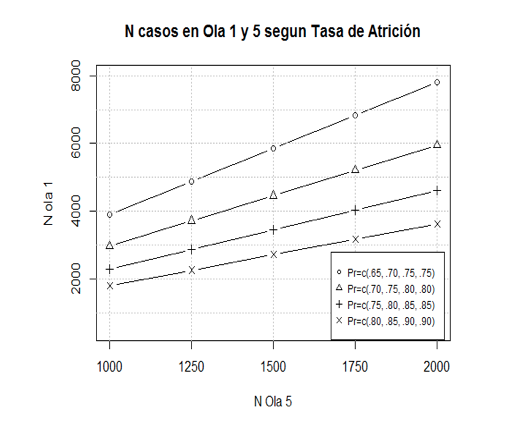
\includegraphics[width=15cm,height=10cm]{attrition_01}
	\end{center}
\end{figure}

El Cuadro \ref{table:attrition_02} describe la recuperación de casos en ELSOC 2017, desagregando en subrgupos claves. Tal como puede observarse, la muestra de 2017 equivale a un 84.49\% de la original, resultado mejor a las estimaciones de un 20\% de atrición en la primera ola. Luego, se observan diferencias sustantivas en términos de sexo y región de locación del entrevistado. \\

\begin{table}[H]
	\centering
	\caption{Análisis de Atrición según Atributos Claves}
	\label{table:attrition_02}
	\begin{tabular}{l c c c }
		\toprule
		\textbf{Variable} & \textbf{Casos 2016} &\textbf{Casos 2017}&\textbf{Recuperación}\\
		\midrule
		\textbf{Total} & 2984 & 2520 & 84.49\%\\
		\midrule
		Hombre & 1191 & 965 & 81.02\%\\
		Mujer & 1793 & 1556 & 86.78\%\\
		\midrule
		Tarapacá & 46 & 46 & 100.00\%\\
		Antofagasta & 61 & 55 & 90.16\%\\
		Atacama & 117 & 95 & 81.20\%\\
		Coquimbo & 147 & 124 & 84.35\%\\
		Valparaíso & 545 & 428 & 78.53\%\\
		R. Metropolitana & 915 & 763 & 83.39\%\\
		OHiggins & 103 & 92 & 89.32\%\\
		Maule & 205 & 190 & 92.68\%\\
		Biobío & 486 & 420 & 86.42\%\\
		Araucanía & 229 & 195 & 85.15\%\\
		Los Ríos & 49 & 45 & 91.84\%\\
		Los Lagos & 58 & 50 & 86.21\%\\
		Aysén & 23 & 18 & 78.26\%\\ 

		\bottomrule
	\end{tabular}
\end{table}


Según el plan de trabajo contemplado por COES, durante el 2018 se levantará la tercera ola de ELSOC. En esta tercera ola se volverá a entrevistar a las personas encuestadas en la primera ola (2016), donde además se integrará una muestra de refresco de 1400 casos. El objetivo de la muestra de refresco es corregir la subcobertura de ciertos grupos poblacionales y ajustar por la pérdida de casos dado la atrición. Los resultados de la tercera ola estáran disponibles durante el primer semestre del 2019. \\

\begin{figure}[H]
	\begin{center}
		\caption{Diseño Muestral de ELSOC según Ola}
		\label{fig:sample}
		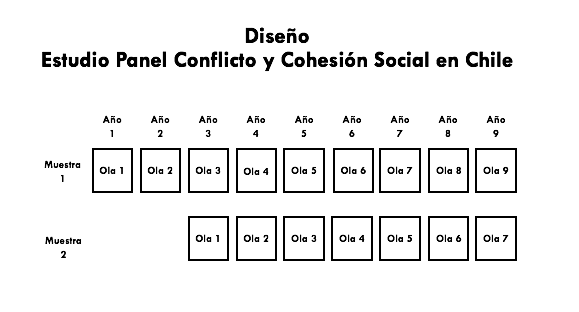
\includegraphics[width=15cm,height=7cm]{Sample_Design}
	\end{center}
\end{figure}


%----------------------------------------------------------------
\newpage
\section*{Registro de Versiones Base de Datos}
\addcontentsline{toc}{section}{Registro de Versiones Base de Datos}

Las versiones adjuntadas de la base de datos, como el presente Manual de Usuario fueron elaborados por el Equipo de Encuestas COES. Sin embargo, \textbf{no pueden ser consideradas como definitivas}, si no que como un primer producto que se pone a disposición de la Comunidad COES. Se desarrollarán nuevas versiones de la base de datos como del Manual de Usuario, de modo de cumplir con la planificación propuesta. 
\textbf{Ni las bases de datos ni el Manual pueden ser entregados a terceros que no sean parte de COES}. Los datos y documentos deben ser obtenidos desde el sitio oficial del estudio.\\

En esta sección se resumen las versiones existentes, a la fecha, de la base de datos correspondiente a la primera segunda del estudio longitudinal (Ver Cuadro \ref{tab:versiones}). A su vez, se reseñan las diferencias entre dichas versiones y los cambios introducidos.\\

\subsection*{Casos Falsificados}

Durante la realización del trabajo de campo de ELSOC 2018, el equipo de Centro Micro Datos, junto al equipo de Encuestas COES detectó que 47 entrevistas correspondientes a la ola 2016 fueron falsificadas. Producto de lo anterior, dichas respuestas fueron eliminadas de la base de datos en la versión 3.0 del 28 de Diciembre de 2018. El problema representa menos del 1\% del tamaño muestral original y, en los análisis realizados por el equipo de Encuestas COES, no se detectaron cambios sustantivos en la distribución de las variables tras su eliminación. \\

\newpage
\begin{table}[H]
	\centering
\caption{Versiones de Base de Datos ELSOC Ola 2 (2017)}
\label{tab:versiones}

\begin{tabular}{c c c l}
\toprule
\textbf{Versión}&\textbf{Fecha}&\textbf{Nombre Archivo}&\textbf{Características}\\
\midrule
\multirow{4}{*}{0.0}&\multirow{4}{*}{27/11/2017}&\multirow{4}{*}{ELSOC Ola 2}& Base original entregada por Centro\\
&&&Micro Datos a COES. Contiene\\
&&&respuestas de 2520 entrevistados (N \\
&&&final) a preguntas del cuestionario.\\
\cdashlinelr{1-4}
\multirow{3}{*}{0.1}&\multirow{3}{*}{12/02/2018}&\multirow{3}{*}{ELSOC Ola 2 Corregido}&Base de datos ajustada a solicitudes\\
&&& de COES, incluyendo chequeos de datos \\
&&&y entrega de bases adicionales\\
\cdashlinelr{1-4}
\multirow{4}{*}{1.0}&\multirow{4}{*}{16/04/2018}&\multirow{4}{*}{ELSOC\_W02\_v1.00}&Base de datos elaborada por COES\\
&&& uniendo información adicional CMD. \\
&&& Con controles de calidad y ajustes a\\
&&& nombres de variables (homologamiento).\\

\cdashlinelr{1-4}
\multirow{4}{*}{2.0}&\multirow{3}{*}{28/12/2018}&\multirow{3}{*}{ELSOC\_W02\_v2.00}&Base de datos elaborada por COES\\
&&& con correcciones introducidas \\
&&& tras eliminación de 47 entrevistas\\
&&& falsificadas.\\

\bottomrule
\end{tabular}
\end{table}

\newpage
\subsection*{Protocolo de Uso de Base de Datos}
\addcontentsline{toc}{section}{Protocolo de Uso de Base de Datos}

Desde la liberación de la base de datos de ELSOC COES Ola 2, éstos se encuentran bajo un período de embargo, por lo que el acceso de la comunidad académica general se encuentra restringido. Los datos se irán liberando de manera modular durante el año 2018, en la medida que se realizan las presentaciones de éstos. Concluido lo anterior, se liberará la base de datos completa. Los datos de ELSOC \textbf{sólo pueden ser utilizados con fines de docencia y/o investigación}. En caso de que se deseen utilizar para otros fines, es necesario solicitar autorización expresa al Equipo de Encuestas de COES. A su vez, cualquier publicación que incluya para su realización el uso de la base de datos (en cualquiera de sus versiones) de los datos del ELSOC debe citar la fuente de la siguiente forma:\\

\vspace{0.3cm}
\noindent \fbox{
	\parbox{\textwidth}{
		Centro de Estudios de Conflicto y Cohesión Social (2018). Estudio Longitudinal  Social de Chile, Primera Ola (ELSOC\_W02\_v2.00) . [Archivo de datos]. Santiago, Chile: Centro de Estudios de Conflicto y Cohesión Social (COES). \url{www.coes.cl}}
}\\
\vspace{0.3cm}

Por último, en caso de que se desee citar el presente Manual de Usuario 
\vspace{0.3cm}

\noindent \fbox{
	\parbox{\textwidth}{
		Centro de Estudios de Conflicto y Cohesión Social (2018). Manual de Usuario de Estudio Longitudinal  Social de Chile, Segunda Ola (2017). Corte Transversal. Versión 2.0. Santiago, Chile: Centro de Estudios de Conflicto y Cohesión Social (COES).}
}\\

\subsection*{Dudas y Consultas}
\addcontentsline{toc}{section}{Dudas y Consultas}

En caso de que detecte problemas con la base de datos, desee plantear solicitudes y/o tenga dudas sobre aspectos no cubiertos por el presente Manual de Usuario, las cuales no puedan ser resueltas por otros medios, puede comunicarse con el Equipo de Encuestas COES al correo electrónico \href{encuestacoes@gmail.com}{encuestacoes@gmail.com}.
El equipo procesará su solicitud y tratará de contestar en el más breve plazo.\\


%----------------------------------------------------------------
\newpage
\section*{Libro de Códigos Base de Datos ELSOC Ola 2017}
\addcontentsline{toc}{section}{Libro de Códigos Base de Datos ELSOC Ola 2017}

Para un uso adecuado de la base de datos de la primera ola de ELSOC COES se recomienda a los investigadores trabajar con el libro de códigos, el cual se presenta a continuación. Este apartado detalla el fraseo de cada uno de los ítemes incluidos, las distintas categorías de respuestas asociadas a éste, y el nombre de las variables como las etiquetas incorporadas en la base de datos. Ahora se incorporan recomendaciones generales para el uso de la base de datos y los libros de códigos.\\


\subsection*{Variables ELSOC Ola 2}
\addcontentsline{toc}{subsection}{Variables ELSOC Ola 2}

La base de datos de ELSOC Ola 2 (2017) contiene una fila por cada entrevistado (son 2520 casos) y una columna por cada variable. Las variables corresponden a los items incluidos en el cuestionario del estudio. Ahora, es necesario que el usuario comprenda plenamente qué es un  ítem. \\

La Figura  \ref{fig:item} presenta, a modo de ejemplo, la pregunta M31 del cuestionario de ELSOC, dónde se consulta a los entrevistados si posee alguno de los siguientes bienes y servicios. En esta pregunta, se incluyen 4 items distintos, correspondientes a cada uno de los cuatro bienes o servicios. En el ejemplo, el primer ítem corresponde a: ``Conexión a TV cable o satelital". Cada ítem corresponde a una variable incluida en la base de datos. El nombre de las variables de la base de datos se construye combinando:\\
\begin{itemize}
	\item El código de la variable en el cuestionario, en letras minúsculas (en el ejemplo corresponde a m31).
	\item Valores numéricos correlativos al orden de los ítems, tal como aparecen en el cuestionario (01, 02, 03 y 04), separado por un guión bajo \_ (en el primer caso, sería m31\_01) .
\end{itemize}

\begin{figure}[H]
	\begin{center}
	\caption{Ejemplo de Pregunta con Múltiples Ítemes en ELSOC}
	\label{fig:item}
		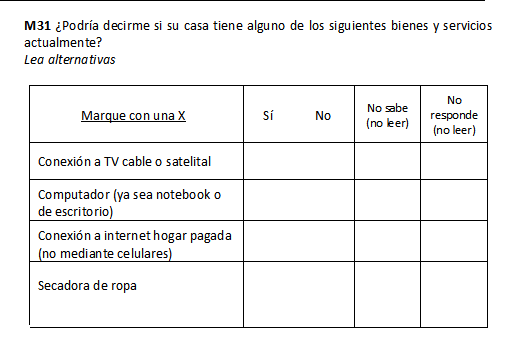
\includegraphics[width=15cm,height=7cm]{Figura_item}
	\end{center}
\end{figure}

El libro de códigos fue diseñado de modo de que sintetice toda la información relevante sobre las variables de la base de datos en un formato común para facilitar su uso. De manera genérica, las variables incluidas en la base de datos tienen el siguiente formato:\\


\noindent \fbox{
	\parbox{\textwidth}{
		\textbf{variableenbase} Fraseo completo de  la pregunta y/o el ítem. Incluyendo instrucciones específicas a éste. \textit{[Etiqueta de variable]}\\
		\vspace{0.1cm}\\
\begin{tabular}{l l l l}
	1&  Etiqueta categoría de respuesta 1 & Frec. Absoluta de 1 & \% correspondiente a 1\\
	2&  Etiqueta categoría de respuesta 2 & Frec. Absoluta de 2 & \% correspondiente a 2\\
	...&...&...&...\\
\end{tabular}		
	}
}
\vspace{0.1cm}\\

A continuación, se presenta un ejemplo para clarificar dicha estructura. En este caso, \textbf{t2\_01} es el nombre de dicho item del cuestionario en la base de datos (como variable). Por medio de estos códigos se pueden identificar los distintos ítemes incluidos. \textbf{Se recomienda rastrear las variables en el Libro de Códigos y en la base de datos según dicho nombre.}  Junto a este código aparece la etiqueta de variable incluida en la base de datos ELSOC. En este caso es \textit{Este es el barrio ideal para mí}. Las etiquetas fueron diseñadas por el equipo ELSOC con el objetivo de describir de modo sucinto el fenómeno o dimensión a medir\footnote{Se intenta preservar el ítem original. Los cambios introducidos se hicieron por motivos de espacio.}, eliminando tildes y otros símbolos no incluidos en todos los softwares estadísticos (por ejemplo, la ñ).

Los distintos valores listados corresponden a las categorías de respuesta asociadas al ítem. En la construcción de la base de datos, dichas categorías fueron ingresadas como valores numéricos y se incluyeron etiquetas de valores. En el ejemplo anterior, si una persona se manifiesta totalmente en desacuerdo con el enunciado, en la encuesta a su respuesta se le asignará un valor numérico de 1, por lo que se podrán realizar operaciones aritméticas con esta respuesta. De todos modos, se incluye una etiqueta para indicar que el valor 1 corresponde con la respuesta ''Totalmente en desacuerdo''.\\

\noindent \fbox{
	\parbox{\textwidth}{
		\textbf{t2\_01} \textit{Este es el barrio ideal para mi}\\
		A continuación voy a leer algunas afirmaciones acerca de su barrio. ¿Qué tan de acuerdo o en desacuerdo está usted con las siguientes afirmaciones?  (MOSTRAR TARJETA 2) Este es el barrio ideal para mí. \\
		\vspace{0.1cm}\\
		\begin{tabular}{l l l l}
			
			1&Totalmente en desacuerdo       & 118 & 3.95\\
			2&En desacuerdo                  & 419 & 14.04\\
			3&Ni de acuerdo ni en desacuerdo & 399 & 13.37\\
			4&De acuerdo                     & 1621& 54.32\\
			5&Totalmente de acuerdo          & 426 & 14.28\\
			8& No sabe (no leer)             & 1   & 0.03\\
			9& No responde (no leer)         & 0   & 0.00\\
		\end{tabular}		
	}
}
\vspace{0.1cm}\\



Por último, es importante también tener en cuenta la información no incluida en este libro de códigos. \textit{``A continuación voy a leer algunas afirmaciones acerca de su barrio. ¿Qué tan de acuerdo o en desacuerdo está usted con las siguientes afirmaciones?"} corresponde la fraseo exacto de la pregunta, \textit{(MOSTRAR TARJETA 2)} aparece entre paréntesis y corresponde a una instrucción para el encuestador. Estos elementos son incluidos de manera completa en el Cuestionario y el Listado de Variables correspondiente.\\

Las variables que poseen categorías residuales de no respuesta (No Sabe y No Responde), generalmente se codifican como 8/9 o 88/99, dependiendo de la anchura de la variable. \textbf{La base de datos de ELSOC 2017 homologa todos las respuestas No Sabe a -888 y No Responde a -999} y chequea la naturaleza de los valores perdidos restantes (los cuales corresponden en su totalidad a la aplicación de filtros). Las respuestas No Sabe y No Responde no fueron eliminadas ni transformadas en valores perdidos en la base de datos,  de modo que los usuarios deben decidir qué hacer con dichos valores de respuesta. La etiqueta de valores de éstos incluye la instrucción de no ser leídos por el encuestador. En el caso de que la pregunta contenga un filtro, los valores no relevantes (filtrados) aparecen en la última línea y no tienen asignado valores ni etiquetas (son valores perdidos por el sistema).\\

Las variables de cadena (texto) no presentan códigos, ya que presentan los verbatim literales de las menciones por parte de los encuestados. El único cambio introducido -y fue realizado por motivos de compatibilidad entre softwares- fue la eliminación de símbolos tales como tildes, diéresis y otros caracteres especiales. A continuación se presenta el ejemplo de una de dichas preguntas:\\

\noindent \fbox{
	\parbox{\textwidth}{
		\textbf{c12\_09esp} A continuación le voy a leer una lista de organizaciones voluntarias. Para cada una de ellas, ¿podría decirme si es miembro activo, miembro inactivo, o no es miembro de estas organizaciones? \textbf{Otra, especifique:} \textit{[Especifique]}\\
		\vspace{0.1cm}\\
		Variable de Cadena (caracteres).
		\vspace{0.1cm}\\
	}
}
\vspace{0.1cm}\\

En el caso de los ítems dónde se pide una respuesta numérica tampoco existen categorías de respuesta, registrándose el valor indicado por el entrevistado. De todos modos se incluyen etiquetas de valores para los valores perdidos. A continuación, un ejemplo de un ítem de este tipo:\\

\noindent \fbox{
	\parbox{\textwidth}{

		\textbf{m37\_01} ¿Cuántos hijos hombres e hijas mujeres ha tenido usted en su vida? (Anote el número respectivo:) 1) Número de hijos hombres. \textit{[Numero de hijos hombres:]}\\
				\vspace{0.1cm}\\
		Respuesta Numérica\\
		88\hspace{0.8cm}   No sabe\\
		99\hspace{0.8cm}   No responde\\
				\vspace{0.1cm}\\
	}
}
\vspace{0.1cm}\\

\subsection*{Características Base de Datos ELSOC Ola 2017}
\addcontentsline{toc}{subsection}{Características Base de Datos ELSOC Ola 2017}

La versión actual de la base de datos (1.0) contiene información 
para los 2520 entrevistados (N definitivo tras supervisión) en relación a los 317 items del cuestionario (cada una corresponde a una variable en la base de datos) y un conjunto adicional de variables:

\begin{enumerate}
	\item \textbf{Identificadoras de Casos:} id de la encuesta, comuna de residencia y región de residencia. 
	\item \textbf{De Diseño Muestral Complejo:} ponderadores (y factores de expansión), estrato y segmento para incorporar el diseño complejo de la encuesta. 
\end{enumerate}

Dentro de las variables de diseño muestral complejo, el estrato identifica a los seis previamente definidos\footnote{Los estratos 4, 5 y 6 tienen sub-estratos Norte y Sur.}: Gran Santiago (1), Gran Valparaíso (2), Gran Concepción (3), Ciudades Grandes(4), Ciudades Medianas (5) y Ciudades Pequeñas (6). La variable segmento1 representa las manzanas/bloques, pero los valores son artificiales (generados por MicroDatos y no corresponden a los valores reales) de modo de garantizar la privacidad de los entrevistados.\\


\vspace{0.3cm}
\noindent \fbox{
	\parbox{\textwidth}{
	\textbf{Se recomienda la utilización de los ponderadores muestrales que ajustan en base a la probabilidad de selección, no respuesta y población objetivo estimada a nivel regional. El ponderador 02 también ajusta en base a la población estimada según sexo.}
	}
}\\
\vspace{0.3cm}

Aún no se encuentran disponibles en la base de datos las variables georreferenciadas que proveerá el Centro de Inteligencia Territorial (CIT), siendo esto motivo de una nueva versión de la base de datos. Esto implicará un nuevo lanzamiento de la base de datos y todas las facilidades para que los investigadores hagan un uso óptimo de las variables territoriales.\\

Las bases de datos se encuentran disponibles en formatos .dta (compatibles con versiones Stata 13 y 14), .sav (compatibles con SPSS) y .RData (compatibles con R, los objetos contienen como atributos etiquetas de variables y valores). El Equipo de Encuestas COES también cuenta con bases de datos adicionales sobre la encuesta (en formato .dta y/o .xlsx):\\
\begin{enumerate}[noitemsep]

	\item Casos supervisados.
	\item Capacitaciones a encuestadores.
	\item Duración de entrevistas.
	\item Códigos de disposición final muestra completa.
	\item Diseño y selección muestra.
	\item Tabla Kish.
	\item Construcción de ponderadores.
\end{enumerate}

Sin embargo, los archivos anteriormente listados deben ser solicitados al Equipo de Encuestas, justificando el uso que se darán a los datos requeridos. El Equipo de Encuestas COES decidirá la pertinencia de dichas solicitudes y se reserva el derecho para entregar dichos datos. \\




\end{document}